%!TEX root = ../report.tex

\begin{document}
    \chapter{Task 4}
    \section{Deliverables }
    \begin{itemize}
        \item[] Extend your report by describing the calibration process, including a theoretical part that describes the camera and lens errors measured and corrected by the calibration. The report should cover:
    \end{itemize}
    
    \begin{itemize}
        \item[1.] A description of the setup for calibration, including possible pitfalls
        \item[2.] An estimation of the number of images and image positions required
        \item[3.] A description of the intrinsic and extrinsic parameters (what do they mean?) calculated by the chosen calibration toolbox
        \item[4.] Discuss possible problems or error sources that can disturb the calibration process. Include any observation you may have made while testing the proper functioning of the camera with your laptop
        \item[5.] Describe the images poses used for calibration and report the found camera parameters including any error estimates (where applicable)
    \end{itemize}
    
    \section{Description of set up}
    
    Camera calibration is carried out to estimate the intrinsic and extrinsic parameters of the camera and lens combination. Described below are the setup and the process carried out for calibration.
    
    \subsection{The set up}
  We were provided with a Basetech SC626 web camera that captures images with a 640x480 pixel for this experiment.
  We quickly had to realize, that the cameras own attachment was too loose and we could not fix it properly to any surfaces or tripods. Since we wanted do have it fixed in one position, we had to improvise.
     
    Our solution was to disassemble the attachment by unscrewing it and used a countersunk m1.7 screw to fix it onto a short aluminium profile. This allowed us to use clamps for a solid attachment onto a shelve. See \ref{fig:camera_setup1} for a overview and \ref{fig:camera_setup2} for a zoomed in view.
    
    \begin{figure}[H] 
            \centering
            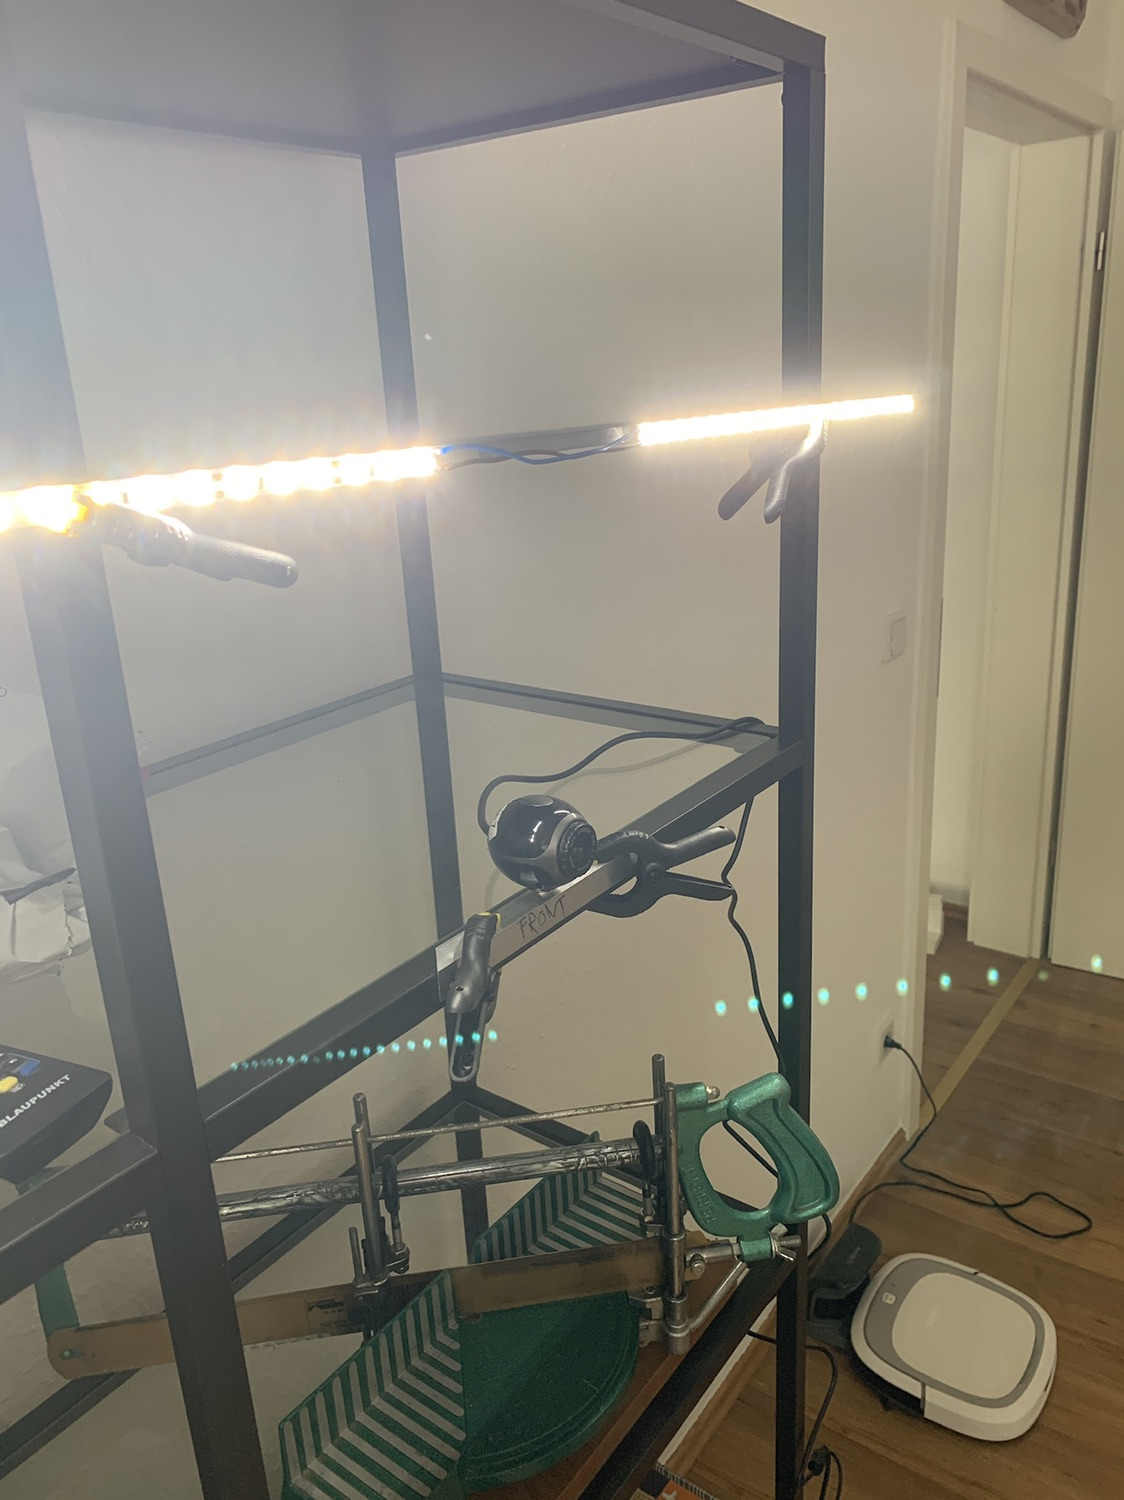
\includegraphics[scale=0.17]{images/experiment_4/IMG_1321.jpg}
              \caption{Camera setup}
            \label{fig:camera_setup1}
     \end{figure}
     
         \begin{figure}[H] 
            \centering
            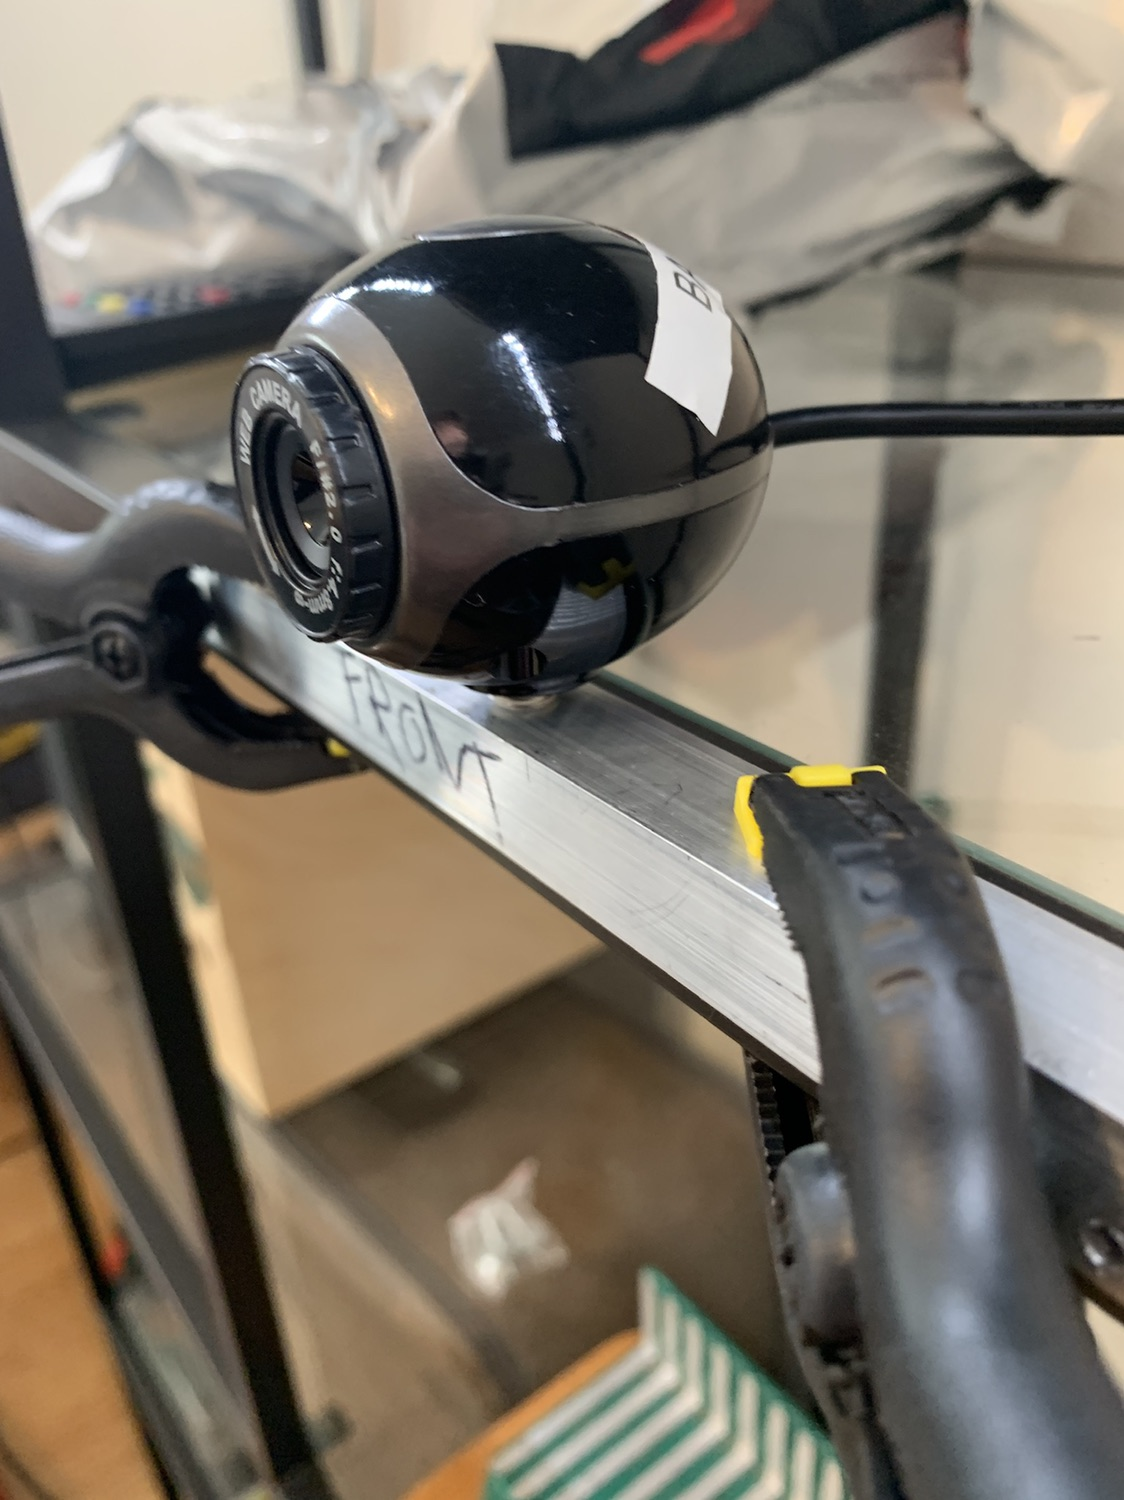
\includegraphics[scale=0.17]{images/experiment_4/IMG_1324.jpg}
              \caption{Camera setup close up}
            \label{fig:camera_setup2}
     \end{figure}
     
      \begin{figure}[H] 
            \centering
            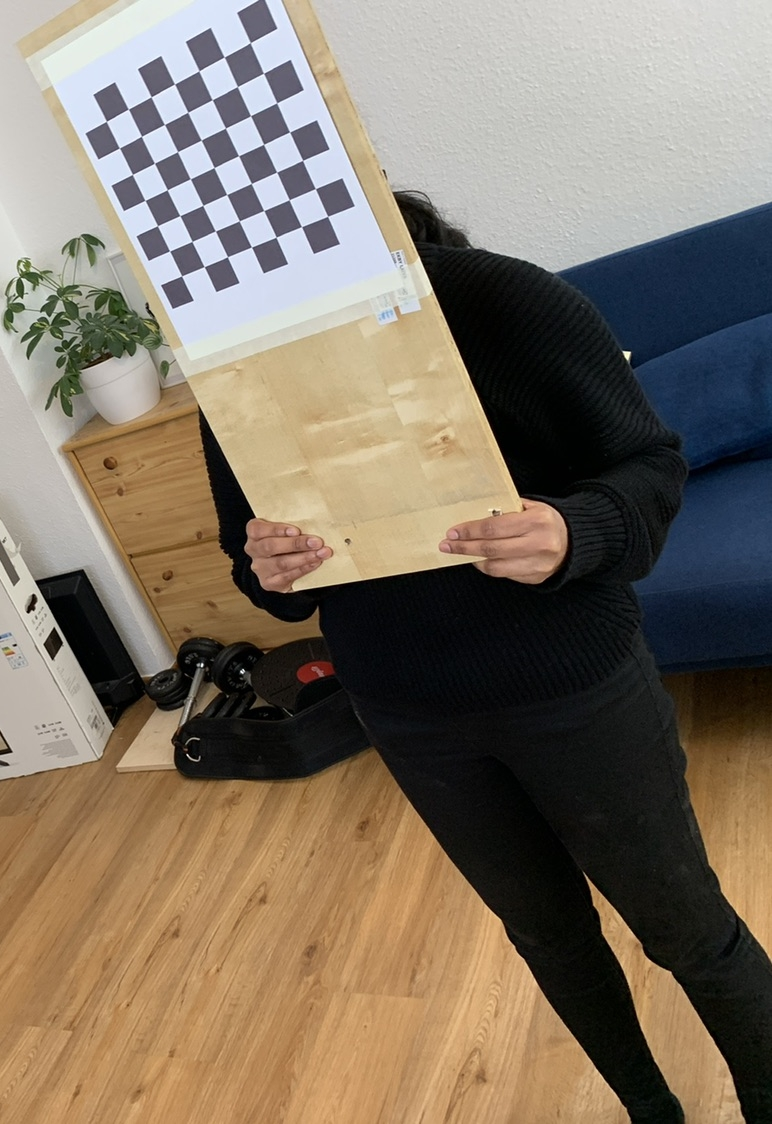
\includegraphics[scale=0.2]{images/experiment_4/IMG_1327.jpg}
              \caption{Checkerboard pattern on the plank}
            \label{fig:camera_setup3}
     \end{figure}
     
    Since the camera had really bad quality and was highly depended on the ambient lighting, we used parts of a full-spectrum daylight (5500k) led strip attached to another aluminium profile. This made sure that the lightning good enough for consistent pictures Figure (\ref{fig:camera_setup1}).
     
    As a next step, we printed the checkerboard pattern for calibration onto an A4 sheet. For stability reasons we used masking tape to fix it to a wooden plank. This allowed better handling and stopped the paper from wrinkling and other deformations, making sure the calibrations pattern lies on a single flat plane(making the assumption z=o on the surface of the pattern to be more accurate which is necessary for calibration) and will make the calibration results more accurate. see \ref{fig:camera_setup3}.
    
    \subsection{The calibration process}
    \begin{itemize}
        \item[1.] First a chessboard pattern was selected, downloaded and printed on a piece of A4 sheet paper. 
        \item[2.] The pattern was then pasted on top a wooden plank as show in the Figure \ref{fig:camera_setup3}. 
        \item[3.] Auto focus was disabled and the resolution was set to the highest possible in the camera(640x320 in the case of our camera).
        \item[4.] Then, pictures were taken at various orientations and distances from the camera. The default image capture software on Ubuntu 18.04 called "Cheese"  was used to capture the images. Only the ones which are in focus, 26 of them were used for further processing. The references provided on the manual for practical experiments recommended minimum of 10 but we took 26 (as it was also stated in the experimentation manual)for better results and to see what kind of extreme views will make it difficult for the algorithm to find corners. The pictures were taken so that the calibration pattern was rotated about all three of its axis.
        \item[5.] Calibration target was detected and the parameters are computed. Details of which are given below.
    \end{itemize}
    
    \section{Description of calibration parameters}
    
        \begin{itemize}
            \item When a camera observes the 3D world it only sees the projection of the 3D world as 2D image on its sensor. The pinhole camera model  given in Figure            \ref{fig:pin_hole_cam_model} is considered to be an good approximate for this model.
            
            \begin{figure}[H] 
                \centering
                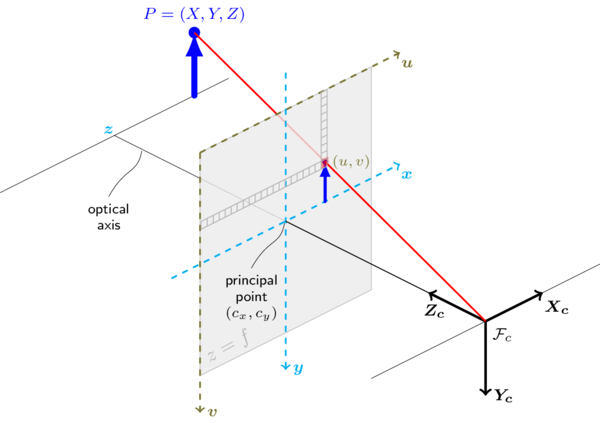
\includegraphics[width=10cm]{"images/experiment_4/pinhole_camera_model.png"}
                \caption{Pin Hole Camera Model \cite{2014opencv} }
                \label{fig:pin_hole_cam_model}
            \end{figure}
                 
                 
            \item  Using the  Figure \ref{fig:pin_hole_cam_model} as a model the mathematical description of the 3D world coordinates transformed to the 2D image coordinate system         can be described as below
                                            
                                            $$ S\begin{bmatrix} U\\ V \\ 1 \end{bmatrix}=  
                                                \begin{bmatrix} \alpha & \gamma & u_0 \\ 
                                                                0 & \beta & v_0       \\ 
                                                                0 & 0& 1
                                                \end{bmatrix}
                                                \begin{bmatrix} r_{11} & r_{12} & r_{13} & t_1 \\
                                                                r_{21} & r_{22} & r_{23} & t_2 \\ 
                                                                r_{31} & r_{32} & r_{33} & t_3 
                                                \end{bmatrix}  
                                                \begin{bmatrix} X\\ Y \\ Z \\ 1 \end{bmatrix}
                                            $$
         
            \item   The above model can be expressed in the compact form as given below
                    $$sm'=A[R|t]M'$$
                    
                    
            \item        The following notations were used:
                            \begin{itemize}
                                \item (X, Y, Z): Coordinates of a 3D point in the world coordinate space \textcolor{blue}{(measured in meters)}
                                \item (u, v)   : Coordinates of the projection on sensor in pixels (image coordinate system)
                                \item A        : Matrix containing intrinsic parameters of camera
                                \item $u_0$, $v_0$  : Coordinates of principle point(usually mid point of image) \textcolor{blue}{in pixels}. Also represented as $c_x$ and $c_y$ respectively
                                \item $\alpha$, $\beta$ : focal length along x and y in pixels respectively
                                \item $\gamma$ : Skew angle between u and v axes (usually 0) in \textcolor{blue}{radians}
                                \item s : scaling factor
                                \item m' : Augmented u,v matrix (image coordinate) in pixels
                                \item M' : Augmented X, Y, Z matrix(world coordinate) in meters
                                \item R  : Rotation of image with respect to world coordinate in \textcolor{blue}{radians}
                                \item t  : Translation of image with respect to world coordinate \textcolor{blue}{in meters}
                                
                            \end{itemize}
                            
            \item The most important point to remember is that there are three individual coordinate systems involved here.  
            
                \begin{enumerate}
                    \item The world coordinate system represented by M' in meters
                    \item The camera coordinate system found by $[R|t]M'$
                    \item The image coordinate system m' found by $A[R|t]M'$
                \end{enumerate}
                
            \item The matrix M' contains $\begin{bmatrix}X&Y& Z& 1\end{bmatrix}^T$  the world coordinates while matrix m' represent the $\begin{bmatrix}U& V & 1\end{bmatrix}^T$ the image coordinates. The matrices R and T describe the transformation of world coordinate system to camera coordinate system. An multiplying the resulting matrix by A matrix will transform the world coordinates to image coordinate system
            
            \item The matrix A which represent the intrinsic parameters of the camera is unique for a given camera and lens combination setup given that the focal length does not change.
                \begin{enumerate}
                    \item The $\gamma$ value which represent the skew angle between U and V axes is usually taken as 0 . (OpenCV library does this by default)
                    \item The $u_0$ and $v_0$ are the principle points of the image plane a good estimate would be the center of the image frame. Given our camera has 640x480 a good estimate would be $u_0=320$ and $v_0=240$ 
                \end{enumerate}
            
            \item The value S is an arbitrary scaling factor for a given image
            
            
            \item  Furthermore an image obtained from the camera will be distorted due to defects of the lens. These can be  categorized mainly into two  types
                        
                        
                        \begin{itemize}
                            \item Tangential distortion: Tangential distortion occurs when the lens is not along its image axis (along the length with the imaging plane). This makes the image appear stretched longer or tilted distorting the perception of depth of the image. 
                            p1 and p2 are coefficients that represent the tangential distortion. 
                            
                            \item Radial Distortion: This is the most common type of distorting which make the image look like its bulged out or pulled in the middle . There are two types of distortions barrel(bulged out) and pincushion(pulled in the middle).
                            This type of distortion make the straight line in real life look curved in the image. Lenses such as fish eye and other wide angle lenses have a significant radial distortion. While web cameras such as the one we use have much smaller barrel distortion
                             $k_1-k_6$ are radial distortion coefficients
                             If 
                             $k_1>0$ barrel distortion 
                             $k_1<0$ pin cushion distortion
                              
                        \end{itemize}
                        
                        
                        
                \item The following equations can be used to correct for the distortion caused:
                        \newline
                         Radial distortion corrected:
                         $$x_{corrected}=x(1+k_1r^2+k_2r^4+k_3r^6)$$
                         $$y_{corrected}=y(1+k_1r^2+k_2r^4+k_3r^6)$$
                         
                         Tangential distortion corrected:
                         
                         $$x_{corrected}=x+[2p_1xy+p_2(r^2+2x^2)]$$
                         $$y_{corrected}=y+[p_1(r^2+2y^2)+2p_2xy)]$$
                         
                         $$r^2=(\frac{x}{z})^2+(\frac{y}{z})^2$$
                         
                         
                \item    The camera calibration code follows the following steps
                         \begin{enumerate}
                             \item Load the images of chessboard(also called checkerboard pattern)
                             \item Define the 3D coordinates of world coordinate system starting from the surface of the board(therefore Z=0 on the board)
                             \item Convert image to grayscale(make the contrast between corner colours easier to find)
                             \item use findChessboardCorners() function to calculate the image coordinates(u and v) for each 3D point using the vertices of the chessboard Figure \ref{fig:ChessBoardCorners}
                             \item If corners were found use cornerSubPix() function to find subpixel level corner detection for more accurate results
                             \item Use calibrateCamera() function which uses the Zhengyou Zhang algorithm to find the camera parameters
                             \item If required use undistort() function to correct for camera distortions
                         \end{enumerate}
                         
                         
                \item     An important note is that OpenCV function calibrateCamera() return four matrices
                            \begin{enumerate}
                                \item Camera Matrix: The intrinsic parameters of the camera as 3x3 Matrix
                                \item Distortion coefficient  : A vector with distortions parameters in the form [$k_1, k_2, p_1, p_2, k_3$]
                                      An important note  $k_4-k_6$ are ignored in OpenCV and if the vector contains only four elements, it means that $k_3=0$ 
                                      
                                \item Rotating : The rotation of each image w.r.t to the world coordinate system
                                \item Translation : The translation of each image w.r.t to the world coordinate system
                            \end{enumerate}
                            
                \item    The distortion coefficients do not depend on the scene viewed and intrinsic parameters will remain the same for a fixed focal length. This mean we can use these values throughout.
            
        \end{itemize}
   
    
    
    
        
        \subsection{Problems during calibration: error sources}
        \begin{itemize}
            \item Selection of the calibration target: The chessboard pattern was chosen since their corners are rather easier to detect and is usually invariant to lens distortion. Using square grids or circle hexagons can introduce errors due to lens distortion.
            \item The calibration target has to mounted on a flat surface. There will be a decrease in the accuracy of calibration if there is warping.
            \item Pictures taken from the same region can introduce a bias.
            \item Camera being on auto focus as it will cause the focal length to change. In our experiment we made sure the camera was not changing the focus
            \item Insufficient camera resolution. This means the accuracy of the coordinated of the corners found will less
            \item Since we held the calibration pattern by hand the image can move slightly while being captured which could result in some motion blur.
            
            \item The quantitative effect of camera shutter speed and lens aperture size on the accuracy of the parameters is difficult to find.
            
            \item If the borders of the calibration pattern are heavily occluded it is difficult for the algorithm to detect corners. This can be see from our test results.
        \end{itemize}
    
   \section{Results and discussion}\label{Results}
   
   \begin{itemize}
       \item The camera used for this experiment is an Basetech SC626 web cam that captures images with a 640x480 pixel resolution. It has a manually adjustable focus therefore for this experiment we left the focus constant.
       
       \item After running the code given in \nameref{CodeCalibration} the following results were obtained
       \vspace{10px}
       \newline
           Intrinsic Camera Matrix=$\begin{bmatrix} \alpha & \gamma & u_0 \\ 
                                    0 & \beta & v_0       \\ 
                                    0 & 0& 1
                    \end{bmatrix}$=$\begin{bmatrix}788 & 0& 320\\0 &824 & 220\\ 0 & 0 &1
                                    \end{bmatrix}$
                                    
                                    
        \item One observation we can make is that from the algorithm we found $u_0=320$ and $v_0=220$ while we expected it to be $u_0=320$ and $v_0=240$ because the resolution of the camera is 640x480 pixels and the value is usually close to the mid point of the pixel values. Trusting the calibrated values will be more accurate this means the rest of the parameters should also withing acceptable levels.
                                    
        \item Distortion coefficients=$\begin{bmatrix}k_1 & k_2& p_1& p_2&             k_3\end{bmatrix}$=$\begin{bmatrix}0.254 & -3.272 & -0.001 & 0.006 & 11.386
                            \end{bmatrix}$
                            
        \item Having a positive $k_1=0.254$ we can see that there is a small barrel distortion(radial )
                            
                            
        \item An example of chessboard with its corners detected is depicted in Figure \ref{fig:ChessBoardCorners}
            
            \begin{figure}[H] 
                            \centering
                            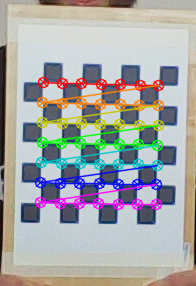
\includegraphics[scale=1.5]{"images/experiment_4/corner_detected.png"}
                            \caption{Detected Corners}
                            \label{fig:ChessBoardCorners}
                     \end{figure}
                     
                     
        \item  While some extreme image orientations did not allow for corner detection. Looking at the images we can see that some of the images make it difficult to distinguish the distances between different places on the checker board. 3 out of the 19 images we used to calibrate were rejected as their corners could not be detected.
                Such as one given in Figure \ref{fig:NoCorners}
    
                \begin{figure}[H] 
                                \centering
                                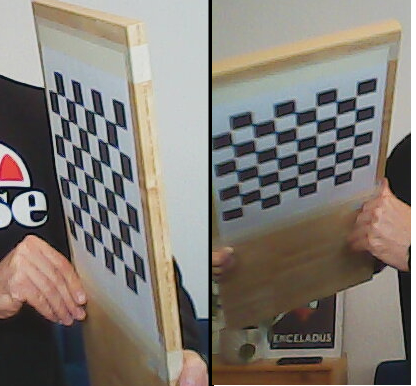
\includegraphics[scale=0.6]{"images/experiment_4/no_corner.png"}
                                \caption{Images corners could not be detected}
                                \label{fig:NoCorners}
                         \end{figure}
                            
        \item  As we can see the parameters are really small and hence the distortion is small . The Figure \ref{fig:correctes_distortion} show an image before(left) and after(right) applying corrections for distortion
    
            \begin{figure}[H] 
                    \centering
                    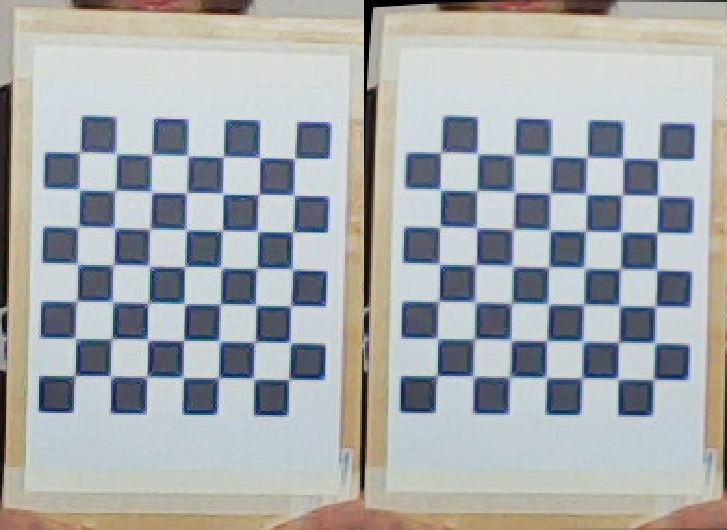
\includegraphics[scale=0.6]{"images/experiment_4/before_n_after_distortion.png"}
                    \caption{Corrected for distortion}
                    \label{fig:correctes_distortion}
             \end{figure}
    
    
        \item The best estimate for the error of these calculated parameter can be found using the re-projection error . The closer error is to o the better the results are. It is found using the L2 norm between the object points found using corner detection and the projected 2d points which were found by transformation of the 3D points to 2D projection using the rotation and translation vectors we find. The average error is found by taking the mean error.
        
        \item For our experiment the mean error is $0.3$ pixels
                            
                            
   \end{itemize}
   
       \subsection{Calibration code}\label{CodeCalibration}
   
       \begin{minted}{cpp}
 
// Open Cv libraries 
#include "opencv2/core.hpp"
#include "opencv2/imgcodecs.hpp"
#include "opencv2/imgproc.hpp"
#include "opencv2/highgui.hpp"
#include <opencv2/calib3d/calib3d.hpp>


//opecv lib for eigen mat conversion. These two need to be imported in this order for this to work
#include <Eigen/Core>
#include <opencv2/core/eigen.hpp> 

//Eigen(cpp equivalent for numpy)

#include "Eigen/Dense"

//Other libraries
#include <iostream>
#include <string>
#include <unistd.h>



//Declare namespaces
using namespace std;
using namespace cv;
using namespace Eigen;




//Global coordinates


int chessboard[2]={7,7};// Size of the chessboard
                        // I assumed our chessboard was 8x8
                        // But apparently not //Dimensions of the checker board 7,7
// Matrix to save test undistorted image
Mat undis_test;


//Function to use 

// The function to stream live camera feed
void stream_camera(int argv);


int main(int argc , char** argv)
{
    
    //  To run the code , type
    //  "./Assignment_3_1" in termnial

    // Since we need to declare a 3D point of the image
    // We define a vector of a vector each element being able 
    // to store 3 floating points that relate images 
    // 2D point to a real world 3D point
    // Unlike arrays size of vectors can increase dynamically
   std::vector<std::vector<cv::Point3f>> objpoints;

   //Create a vector to save 2D point of the chess board image
   vector<vector<cv::Point2f>> imgpoints;

   //The algorithm define the corner of the chess board as the world origin
   // This mean the z=0 for the surface of the chess board

   //Defining the 3D coordinates 
   vector<cv::Point3f > objp;



   for (int i{0}; i<chessboard[1];i++)
   {
       for(int j{0} ; j<chessboard[0];j++)
       {

           //Push back is similar to heap_push. 
           //add a vector to the last position of the array
           objp.push_back(cv::Point3f(j,i,0));
       }
   }


    //Vector to store image file names
    vector<cv::String>images;

    // Path of the folder containing chessboard images
    std::string path = "/home/malika/Documents/Bonn Stuff/SEE/Report/SEE/
    data/Assignment_3_1/calib_images/..jpg";

    //The path to all images for calibration
    cv::glob(path,images);

    //Cv mat to save original and grayscaled images
    cv::Mat original, gray;

    //Vector to store the corners detected on the chess board 
    vector<cv::Point2f> corner_points;

    //Check if finding corners were successful
    bool if_sucess;

    // Window to diplay corners
    namedWindow("Corner_Image", CV_WINDOW_KEEPRATIO);
    //Loop though all image

    

    for(int i{0};i<images.size();i++)
    {
        //load up the image
        original=imread(images[i]);
        //convert to grayscale
        cvtColor(original,gray,CV_BGR2GRAY);        

        //finding corners
        if_sucess=findChessboardCorners(gray,cv::Size(chessboard[0],chessboard[1]),corner_points, 
        CV_CALIB_CB_ADAPTIVE_THRESH | CV_CALIB_CB_FAST_CHECK | CV_CALIB_CB_NORMALIZE_IMAGE);
        
        /*

        Various operation flags that can be zero or a combination of the following values:

        CALIB_CB_ADAPTIVE_THRESH :

        Use adaptive thresholding to convert the image to black and white, rather than a 
        fixed threshold level (computed from the average image brightness).


        CALIB_CB_NORMALIZE_IMAGE:
         Normalize the image gamma with equalizeHist() before applying 
         fixed or adaptive thresholding.


        CALIB_CB_FILTER_QUADS:
         Use additional criteria (like contour area, perimeter, 
         square-like shape) to filter out 
         false quads extracted at the contour retrieval stage.

        CALIB_CB_FAST_CHECK :
        Run a fast check on the image that looks for chessboard corners,
         and shortcut the call if none is found. 
         This can drastically speed up the call in the
          degenerate condition when no chessboard is observed.


        */


       if(if_sucess)
       {

           //Save the first image for pre and post distotion comparison
           if(i==0)
           {
               undis_test=imread(images[i]);
           }

           //Set the termination criteria for fiding corners at subpixel level
           //No of itersatons and accuracy criteria 
           TermCriteria stop_critera(CV_TERMCRIT_EPS| CV_TERMCRIT_ITER,30,0.001);
            
            //Perform the subpixel level corner detection
           cornerSubPix(gray,corner_points,cv::Size(11,11),cv::Size(-1,-1),stop_critera);

           //drawt the found corerns on the original image matrix

           drawChessboardCorners(original,cv::Size(chessboard[0],chessboard[1]),
           corner_points,if_sucess);
           /*
           complete board was found or not. The return value of findChessboardCorners 
           should be passed here. The function draws individual chessboard 
           corners detected either as red circles 
           if the board was not found, or as colored corners 
           connected with lines if the board was found.
            
            */

           // Add the inital known 3d word coorndiated(corner of chess board) 
           // in pair with the corner points found
           objpoints.push_back(objp);
           imgpoints.push_back(corner_points);







           imshow("Corner_Image",original);
           waitKey(20);
       }     

        else
        {            
            cout<<"could not find chess board for "<<images[i]<<endl;
        } 
    }
    destroyAllWindows();
    //CamMat: Camera intrinsic properties
    // dist_coe : camera distortion coeffcients(radial and tangential)
    // R,T : the roatioan and translation wrt cam
    Mat cameraMat,dist_coefficent,R,T;
    /*
    Tangential distortion: Tangential distortion occurs mainly because 
    the lens is not parallely aligned 
    to the imaging plane, that makes the image to be extended a little while longer or tilted, 
    it makes the objects appear farther away or even closer than they actually are.
    p1 n p2 are tangential distortion coefficients

    Radial Distortion: Radial Distortion is the most common type that affects the images, 
    In which when a camera captured pictures of straight lines appeared 
    slightly curved or bent k1-k6 are radial

     k1>0 barrel 
     k1<0 pincusshsion
     In the functions below the coefficients are passed or returned as:
    (k_1, k_2, p_1, p_2, k_3 [, k_4, k_5, k_6])
    k4-k6 are ignored in opencv
     If the vector contains four elements, it means that k_3=0 . 
     The distortion coefficients do not depend on the scene viewed
    */

    calibrateCamera(objpoints,imgpoints,cv::Size(gray.rows,gray.cols),
    cameraMat,dist_coefficent,R,T);
    //Store the length of the Rotation matrix to count no of images used
    cv::Size size_R=R.size();


   double mean_error=0;
    // Reprojection error_calulation

    vector<Point2f> imagePoints2;
    size_t totalPoints = 0;
    double totalErr = 0, err;
    vector<float>perViewErrors;
    perViewErrors.resize(objpoints.size());

  

    for(size_t i = 0; i < objpoints.size(); ++i )
    {
        
        // const double* rvecs = R.ptr<double>(i);
        // const double* tvecs = T.ptr<double>(i);

     
        std::vector<double>rvects;       
        rvects.push_back(R.at<double>(i,0));
        rvects.push_back(R.at<double>(i,1));
        rvects.push_back(R.at<double>(i,2));

        std::vector<double>tvects;       
        tvects.push_back(T.at<double>(i,0));
        tvects.push_back(T.at<double>(i,1));
        tvects.push_back(T.at<double>(i,2));
        // cout << "shortvec = " << Mat(v) << endl;
        projectPoints(objpoints[i], rvects, tvects, cameraMat, dist_coefficent, imagePoints2);        
        err = norm(imgpoints[i], imagePoints2, NORM_L2);
        size_t n = objpoints[i].size();
        totalErr        += err;
        totalPoints     += n;

      
    }

    mean_error=std::sqrt(totalErr/totalPoints);

    std::cout << "cameraMatrix : \n" << cameraMat << std::endl;
    cout<<""<<endl;
    cout << "distCoeffs : \n" << dist_coefficent << std::endl;
    cout<<""<<endl;
    cout<<""<<endl;
    cout<<""<<endl;
    cout << "Rotation vector : \n" << R << std::endl;
    cout<<""<<endl;
    cout<<""<<endl;
    cout<<""<<endl;
    cout << "Translation vector : \n" << T << std::endl;
    cout<<""<<endl;
    cout<<""<<endl;
    cout<<"The no of images used for calibration :"<<size_R<<endl;
    cout<<"Mean Error "<<mean_error<<endl;

    

    //Create an eigen mat and conver the cv mat to eigen for test
    //  MatrixXf eigemat;
    //  cv::cv2eigen(cameraMat,eigemat);
    //  cout<<"The eigne : \n"<<eigemat<<endl;


    //For an example take the first image of the test data and 
    // undistort it to see the affect of distorion
    Mat undistored_out;
    cv::undistort(undis_test,undistored_out,cameraMat,dist_coefficent);
    hconcat(undis_test, undistored_out, undistored_out);
    cvNamedWindow("Before and after undistorion",WINDOW_KEEPRATIO);
    imshow("Before and after undistorion",undistored_out);
    waitKey(0);
    // Test code for Eigen
    // MatrixXd m = MatrixXd::Random(3,3);
    // m=(m+MatrixXd::Constant(3,3,1.2))*50;
    // cout<<"m ="<<m<<endl;
    // char camera_stream;
    // cout<<"Enter name"<<endl;
    // cin>>camera_stream;
    // stream_camera(int(camera_stream));
    return 0;
}
void stream_camera(int c)
{
    cout<<"The cout is "<<c-48<<endl;

    VideoCapture stream1(0);
    Mat frame1;
    namedWindow("Display Image", WINDOW_AUTOSIZE );
    if(!stream1.isOpened()){
            cout <<"Camera not opened" << endl;
        }
        else{
            while(true)
            {
                stream1.read(frame1);
                imshow("Display Image", frame1);
                waitKey(30);
            }
        }
}
        \end{minted}
    

    
    
\end{document}
